% =====================================================================
%  CO3133 Deep Learning and Its Applications -- Assignment 02 slides
%  Group Goat -- Emotion classification on dair-ai/emotion
%  Compile with XeLaTeX (Overleaf: Menu -> Compiler -> XeLaTeX) or Tectonic.
%  Plain Beamer look: Latin Modern font, white background, one dark-blue colour.
%  Every number comes from ../results/ (exported by the notebook) or from
%  the report (report/Goat_A2_Report.tex), which uses the same files.
%  The speaking script is slides/A2_video_script.md.
% =====================================================================
\documentclass[aspectratio=169,10pt,t]{beamer}

\usepackage{fontspec}      % Latin Modern (the standard LaTeX font), Unicode for Vietnamese names
\usefonttheme{professionalfonts}
\usepackage{amssymb,pifont}
\usepackage{appendixnumberbeamer}
\usepackage{booktabs,array,tabularx,colortbl,multirow}
\usepackage{tikz}
\usetikzlibrary{arrows.meta,positioning,fit,calc,shapes.misc,backgrounds}
\usepackage{tcolorbox}
\tcbuselibrary{skins,raster}
\usepackage{qrcode}

% ---------- colours: one dark blue for structure, greys for text ----------
\definecolor{navy}{HTML}{0B2A4A}
\definecolor{ink}{HTML}{1A1A1A}
\definecolor{muted}{HTML}{5F6B7A}
\definecolor{linec}{HTML}{C8CED6}
\definecolor{accent}{HTML}{1769AA}
\colorlet{accentB}{accent}
\colorlet{softblue}{black!4}
\colorlet{softteal}{black!4}
% model colours (same as the training-curve figure), used only for small dots
\definecolor{distilc}{HTML}{2A78D6}
\definecolor{bertc}{HTML}{1BAF7A}
\definecolor{frozenc}{HTML}{EB6834}
\definecolor{basec}{HTML}{7A8797}
\colorlet{newc}{red!8!white}
\colorlet{prec}{black!4}
\definecolor{failc}{HTML}{B91C1C}
\definecolor{okc}{HTML}{15803D}

\hypersetup{colorlinks=true,urlcolor=accent,linkcolor=accent}
\arrayrulecolor{black!45}

% ---------- beamer chrome: plain white, title + rule, simple footer ----------
\setbeamertemplate{navigation symbols}{}
\setbeamersize{text margin left=1.0cm,text margin right=1.0cm}
\setbeamercolor{normal text}{fg=ink,bg=white}
\setbeamercolor{structure}{fg=navy}
\setbeamerfont{normal text}{size=\small}
\setbeamertemplate{itemize items}[circle]
\setbeamertemplate{enumerate items}{\textcolor{navy}{\bfseries\insertenumlabel.}}

\setbeamertemplate{section in toc}{%
  \leavevmode\hbox to 0.75cm{\bfseries\color{navy}\inserttocsectionnumber.\hfill}%
  \textcolor{ink}{\inserttocsection}\par\vskip7pt}
\setbeamertemplate{subsection in toc}{}
\newif\ifbackup
\setbeamertemplate{frametitle}{%
  \nointerlineskip\vskip0.42cm
  \hbox{\Large\bfseries\color{navy}\insertframetitle}%
  \nointerlineskip\vskip5pt
  \hbox{\color{navy}\rule{\textwidth}{0.5pt}}%
  \nointerlineskip\vskip-2pt}

\setbeamertemplate{footline}{%
  \hbox to\paperwidth{\hskip1.0cm\color{muted}\fontsize{6.5}{8}\selectfont
    Group Goat --- CO3133 Assignment 2 \enspace\textperiodcentered\enspace \hyperlink{contents}{\textcolor{accent}{Contents}}\hfill
    \ifbackup Backup\else\insertsectionhead\fi\hfill
    \ifbackup B\insertframenumber\else\insertframenumber\,/\,\inserttotalframenumber\fi\hskip1.0cm}%
  \vskip0.32cm}

% ---------- components ----------
\newtcolorbox{card}[1][]{enhanced,colback=white,colframe=linec,boxrule=0.4pt,arc=1pt,
  left=6pt,right=6pt,top=5pt,bottom=5pt,boxsep=0pt,coltext=ink,fontupper=\small\raggedright,#1}
\newtcolorbox{softcard}[1][]{enhanced,colback=black!4,colframe=black!4,boxrule=0pt,arc=1pt,
  left=6pt,right=6pt,top=4pt,bottom=4pt,boxsep=0pt,coltext=ink,fontupper=\small\raggedright,#1}
\newtcolorbox{banner}[1][]{enhanced,colback=accent!6!white,colframe=navy,boxrule=0pt,leftrule=2pt,arc=0pt,
  left=8pt,right=8pt,top=4pt,bottom=4pt,boxsep=0pt,coltext=ink,fontupper=\small\bfseries,#1}

\newcommand{\ctitle}[1]{\leavevmode{\bfseries\color{navy}#1}\par\vskip3pt}
\newcommand{\eyebrow}[1]{{\scriptsize\bfseries\color{navy}#1}}
\newcommand{\chip}[2][white]{\tikz[baseline=(c.base)]\node[rectangle,draw=linec,fill=#1,rounded corners=1pt,
  inner xsep=3.5pt,inner ysep=1.8pt,font=\scriptsize,text=ink](c){#2};}
\newcommand{\tagc}[2]{\leavevmode{\scriptsize\bfseries\color{navy}#2}}
\newcommand{\mdot}[1]{\tikz[baseline=-0.6ex]\fill[#1](0,0)circle(2.4pt);}
\newcommand{\kpi}[3][]{%
  \begin{card}[halign=left,top=4pt,bottom=4pt]
    {\fontsize{15}{17}\bfseries\color{navy}#2}\par\vskip1pt
    {\scriptsize\color{muted}#3}
  \end{card}}
\newcommand{\yes}{\textcolor{okc}{$\checkmark$}}
\newcommand{\no}{\textcolor{failc}{\ding{55}}}
\newcommand{\eb}{\bfseries}
\newcommand{\sbf}{\bfseries}
\newcommand{\mut}[1]{\textcolor{muted}{#1}}
\newcommand{\quot}[1]{\textit{``#1''}}
\newcolumntype{Y}{>{\raggedright\arraybackslash}X}
\newcolumntype{K}[1]{>{\raggedright\arraybackslash\leavevmode\bfseries}p{#1}}
\newcommand{\hl}{\rowcolor{black!5}}
\newcommand{\thd}[1]{\leavevmode{\bfseries #1}}

\hyphenpenalty=10000 \exhyphenpenalty=10000
\title{Six-Class Emotion Classification}
\author{Group Goat}

\begin{document}

% =====================================================================
%  1. TITLE
% =====================================================================
{\setbeamertemplate{footline}{}
\begin{frame}[plain]
\vskip0.55cm
\centering

\includegraphics[height=1.2cm]{figures/hcmut.png}\par\vskip3pt
{\scriptsize Ho Chi Minh City University of Technology (HCMUT) --- Faculty of Computer Science and Engineering\par}
\vskip3pt
{\footnotesize CO3133 Deep Learning and Its Applications --- Semester 261 --- Assignment 2\par}
\vskip14pt
{\color{navy}\rule{0.8\textwidth}{0.6pt}}\par\vskip8pt
{\LARGE\bfseries\color{navy} Six-Class Emotion Classification\par}
\vskip6pt
{\normalsize A TF-IDF baseline vs.\ fine-tuned DistilBERT and BERT on \texttt{dair-ai/emotion}\par}
\vskip6pt
{\color{navy}\rule{0.8\textwidth}{0.6pt}}\par\vskip14pt
{\small\bfseries Group Goat\par}\vskip3pt
{\small Võ Lê Thành Triệu (2453297) --- presenter\par}\vskip2pt
{\small Hoàng Trọng Huy Minh (2452743) \enspace\textperiodcentered\enspace Nguyễn Huỳnh Nam Quốc (2453089)\par}
\vskip8pt
{\footnotesize\mut{Instructor: Lê Thành Sách}\par}
\end{frame}}

% =====================================================================
%  CONTENTS (every footer links back here; every line links to its section)
% =====================================================================
\begin{frame}[label=contents]{Contents}
\vskip14pt
\begin{columns}[T,onlytextwidth]
\column{0.46\textwidth}
\begin{card}[top=9pt,bottom=3pt]
  \tableofcontents[sections={1-4}]
\end{card}
\column{0.46\textwidth}
\begin{card}[top=9pt,bottom=3pt]
  \tableofcontents[sections={5-8}]
\end{card}
\end{columns}
\vskip10pt
{\scriptsize\mut{Click a section to jump to it; \textcolor{accent}{Contents} in the footer of every slide comes back here. Backup slides (per-class F1, curves, confusion matrices, all 12 runs) follow the last slide.}}
\end{frame}

% =====================================================================
\section{Problem and data}
% =====================================================================
\begin{frame}{One sentence in, one of six emotions out}
\vskip2pt
\begin{columns}[T,onlytextwidth]
\column{0.555\textwidth}
\begin{card}
  \ctitle{The task}
  \footnotesize\renewcommand{\arraystretch}{1.45}
  \begin{tabularx}{\linewidth}{@{}Y@{\hspace{6pt}}c@{\hspace{6pt}}r@{}}
    \quot{im updating my blog because i feel shitty} & $\rightarrow$ & \chip{sadness}\\
    \quot{i felt anger when at the end of a telephone call} & $\rightarrow$ & \chip{anger}\\
    \quot{i find myself in the odd position of feeling supportive of} & $\rightarrow$ & \chip{love}\\
  \end{tabularx}
  \vskip1pt
  {\fontsize{6}{7}\selectfont\mut{Real texts from the test set.}}
\end{card}
\column{0.415\textwidth}
\begin{card}
  \ctitle{Why it is hard}
  \begin{itemize}\setlength{\itemsep}{2pt}
    \item {\sbf Imbalance:} joy has 9.37$\times$ the texts of surprise
    \item {\sbf Close emotions:} joy vs.\ love, fear vs.\ surprise
    \item {\sbf Noisy labels:} same text, two labels
  \end{itemize}
\end{card}
\vskip4pt
\begin{card}
  \ctitle{Metric: Macro-F1 (+ accuracy)}
  {\footnotesize Always predicting \emph{joy}: accuracy {\sbf 0.35}, Macro-F1 {\sbf 0.09} \mut{(test)}}
\end{card}
\end{columns}
\vskip3pt
\begin{banner}
  Question: does fine-tuning a Transformer beat a TF-IDF baseline, and at what cost?
\end{banner}
\end{frame}

% ---------------------------------------------------------------------
\begin{frame}{The data: \texttt{dair-ai/emotion} at a glance}
\vskip2pt
\begin{tcbraster}[raster columns=5,raster equal height,raster column skip=5pt]
  \kpi{20,000}{texts \textperiodcentered{} 16k / 2k / 2k}
  \kpi{6}{classes, one label per text}
  \kpi[frozenc]{9.37$\times$}{joy vs.\ surprise (train)}
  \kpi{17}{median words per text}
  \kpi{0}{texts over 128 tokens (max 87)}
\end{tcbraster}
\vskip5pt
\begin{card}[left=4pt,right=4pt,top=3pt,bottom=3pt]
  \centering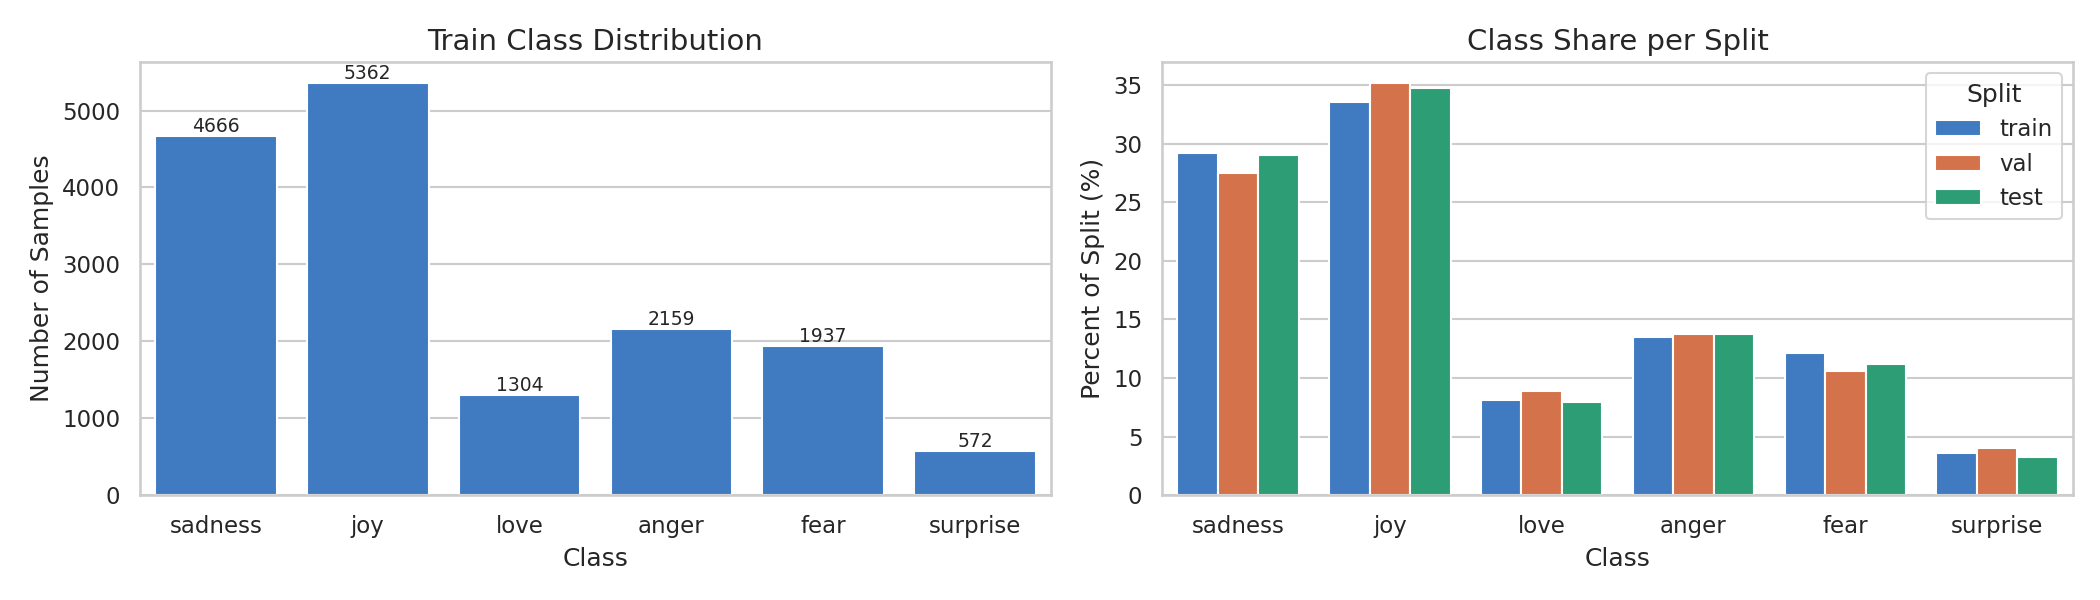
\includegraphics[width=0.93\linewidth,height=4.0cm,keepaspectratio]{figures/a2_class_dist.png}
\end{card}
\end{frame}

% ---------------------------------------------------------------------
\begin{frame}{Cleaning first, so nothing leaks into test}
\vskip3pt
\centering
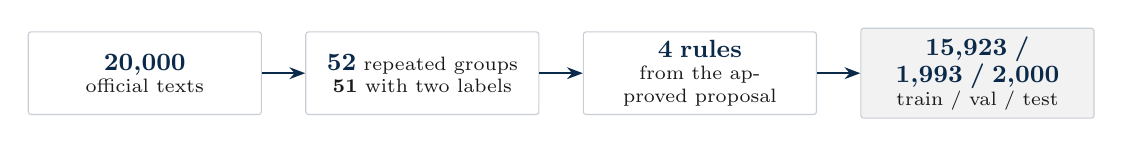
\begin{tikzpicture}[
  st/.style={draw=linec,fill=white,rounded corners=1pt,align=center,font=\scriptsize,text=ink,minimum height=1.05cm,text width=2.75cm,inner sep=3pt},
  ar/.style={-{Stealth[length=2mm]},thick,navy}]
  \node[st] (a) {{\eb\color{navy}\small 20,000}\\official texts};
  \node[st,right=0.55cm of a] (b) {{\eb\color{navy}\small 52} repeated groups\\{\sbf 51} with two labels};
  \node[st,right=0.55cm of b] (c) {{\eb\color{navy}\small 4 rules}\\from the approved proposal};
  \node[st,right=0.55cm of c,fill=black!5,draw=linec] (d) {{\bfseries\color{navy}\small 15,923 / 1,993 / 2,000}\\train / val / test};
  \draw[ar] (a)--(b); \draw[ar] (b)--(c); \draw[ar] (c)--(d);
\end{tikzpicture}
\vskip8pt
\begin{columns}[T,onlytextwidth]
\column{0.53\textwidth}
\begin{card}
  \ctitle{The four rules}
  \begin{enumerate}\setlength{\itemsep}{1pt}\footnotesize
    \item Test stays untouched; its texts are removed from train and val
    \item Text in train and val: drop the train copy
    \item Same text with two labels: drop the whole group
    \item Same text, same label: keep the first copy
  \end{enumerate}
  \vskip2pt
  {\scriptsize\mut{Removed: 77 train, 7 val, 0 test. All 7 checks pass (no overlap, no repeats).}}
\end{card}
\column{0.44\textwidth}
\begin{card}
  \ctitle{Two text versions}
  \footnotesize
  {\sbf Minimal} \mut{(every model)}: Unicode NFC, lowercase, single spaces\par\vskip4pt
  {\sbf Aggressive} \mut{(baseline variant)}: also drops 295 stopwords, {\sbf keeps} \emph{not, no, never, but, very, so \ldots}
\end{card}
\vskip4pt
\begin{softcard}
  \footnotesize\sbf\color{accent}Vocabulary, IDF and class weights are fitted on train only.
\end{softcard}
\end{columns}
\end{frame}

% =====================================================================
\section{Method}
% =====================================================================
\begin{frame}{Three models on one shared pipeline}
\vskip2pt
\begin{tcbraster}[raster columns=3,raster equal height,raster column skip=6pt]
  \begin{card}
    \tagc{basec}{BASELINE}\par\vskip3pt
    \ctitle{TF-IDF + Logistic Regression}
    {\footnotesize Word and word-pair counts, then a linear classifier}\par\vskip5pt
    {\scriptsize\mut{102,426 params \textperiodcentered{} 1.2 MB\\trains in 5.3 s on one CPU}}
  \end{card}
  \begin{card}
    \tagc{distilc}{MAIN MODEL}\par\vskip3pt
    \ctitle{DistilBERT}
    {\footnotesize 6-layer Transformer, every weight fine-tuned}\par\vskip5pt
    {\scriptsize\mut{67.0 M params \textperiodcentered{} 256 MB\\trains in 277 s on a T4 GPU}}
  \end{card}
  \begin{card}
    \tagc{bertc}{COMPARISON}\par\vskip3pt
    \ctitle{BERT}
    {\footnotesize 12-layer Transformer, the same recipe}\par\vskip5pt
    {\scriptsize\mut{109.5 M params \textperiodcentered{} 418 MB\\trains in 525 s on a T4 GPU}}\par\vskip3pt
    {\fontsize{6}{7.5}\selectfont\itshape\color{muted}Added after the proposal: time remained, so we ran it to see what a larger model changes.}
  \end{card}
\end{tcbraster}
\vskip8pt
\centering
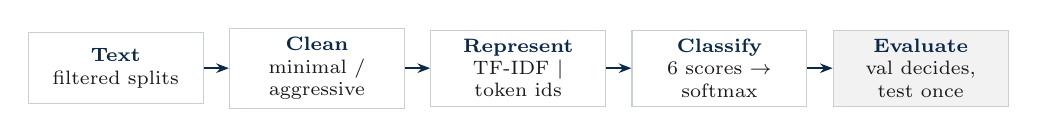
\begin{tikzpicture}[
  sp/.style={rectangle,draw=linec,fill=white,font=\scriptsize,text=ink,
             minimum height=0.9cm,text width=1.8cm,align=center,inner xsep=6pt},
  sp0/.style={sp},ar/.style={-{Stealth[length=1.6mm]},thick,navy}]
  \node[sp0] (p1) {{\sbf\color{navy}Text}\\filtered splits};
  \node[sp,right=0.32cm of p1] (p2) {{\sbf\color{navy}Clean}\\minimal / aggressive};
  \node[sp,right=0.32cm of p2] (p3) {{\sbf\color{navy}Represent}\\TF-IDF \textbar{} token ids};
  \node[sp,right=0.32cm of p3] (p4) {{\sbf\color{navy}Classify}\\6 scores $\rightarrow$ softmax};
  \node[sp,right=0.32cm of p4,fill=black!5] (p5) {{\sbf\color{navy}Evaluate}\\val decides, test once};
  \foreach \a/\b in {p1/p2,p2/p3,p3/p4,p4/p5} \draw[ar] (\a)--(\b);
\end{tikzpicture}
\end{frame}

% ---------------------------------------------------------------------
\begin{frame}{TF-IDF + LR: count features, then a linear classifier}
\vskip0pt
\begin{columns}[T,onlytextwidth]
\column{0.52\textwidth}
\begin{card}
  \ctitle{A toy example: 3 texts, unigrams + bigrams}
  {\fontsize{6.5}{8}\selectfont
  \mut{d1:} feel happy today \enspace \mut{d2:} {\sbf\color{accent}not feel happy} \enspace \mut{d3:} feel scared today\par}
  \vskip3pt
  {\scriptsize
  \renewcommand{\arraystretch}{1.0}
  \begin{tabularx}{\linewidth}{@{}Yccc@{}}
    \toprule
    \thd{n-gram in d2} & \thd{in how many texts} & \thd{IDF} & \thd{weight}\\
    \midrule
    feel & 3 of 3 & 1.00 & \textcolor{muted}{0.32}\\
    happy & 2 of 3 & 1.29 & 0.41\\
    feel happy & 2 of 3 & 1.29 & 0.41\\
    \hl not & 1 of 3 & 1.69 & {\sbf 0.53}\\
    \hl not feel & 1 of 3 & 1.69 & {\sbf 0.53}\\
    \bottomrule
  \end{tabularx}}
  \vskip2pt
  {\fontsize{6.5}{8}\selectfont\mut{IDF $=\ln\frac{1+n}{1+\mathrm{df}}+1$ \quad weight = count $\times$ IDF, then scaled to length 1}}\par\vskip3pt
  {\scriptsize\sbf \textit{feel} is in every text $\rightarrow$ lowest weight;\\ \textit{not} is rare $\rightarrow$ highest weight.}
\end{card}
\column{0.455\textwidth}
\centering
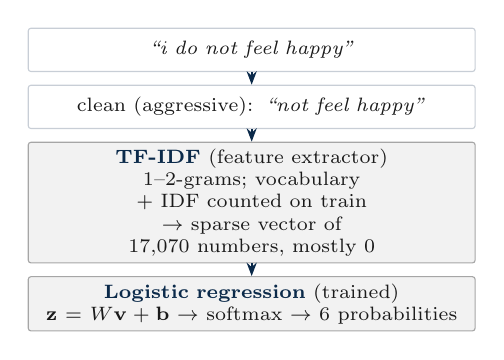
\begin{tikzpicture}[
  bx/.style={draw=linec,fill=white,rounded corners=1pt,align=center,font=\scriptsize,text=ink,text width=5.5cm,inner sep=2.5pt,minimum height=0.55cm},
  fx/.style={bx,fill=black!5,draw=black!35},
  lr/.style={bx,fill=black!5,draw=black!35},
  ar/.style={-{Stealth[length=1.7mm]},thick,navy},
  node distance=0.16cm]
  \node[bx] (t) {\quot{i do not feel happy}};
  \node[bx,below=of t] (c) {clean (aggressive): \quot{not feel happy}};
  \node[fx,below=of c] (f) {{\sbf\color{navy}TF-IDF} (feature extractor)\\1--2-grams; vocabulary + IDF counted on train\\$\rightarrow$ sparse vector of 17,070 numbers, mostly 0};
  \node[lr,below=of f] (l) {{\sbf\color{navy}Logistic regression} (trained)\\$\mathbf{z}=W\mathbf{v}+\mathbf{b}$ $\rightarrow$ softmax $\rightarrow$ 6 probabilities};
  \draw[ar](t)--(c); \draw[ar](c)--(f); \draw[ar](f)--(l);
\end{tikzpicture}
\vskip5pt
\begin{banner}[fontupper=\scriptsize\bfseries]
  TF-IDF is a fixed feature-extraction block: no gradient learning. Only the logistic regression is trained.
\end{banner}
\end{columns}
\end{frame}

% ---------------------------------------------------------------------
\begin{frame}{DistilBERT and BERT: same width, half the depth}
\vskip0pt
\begin{columns}[T,onlytextwidth]
\column{0.70\textwidth}
\centering
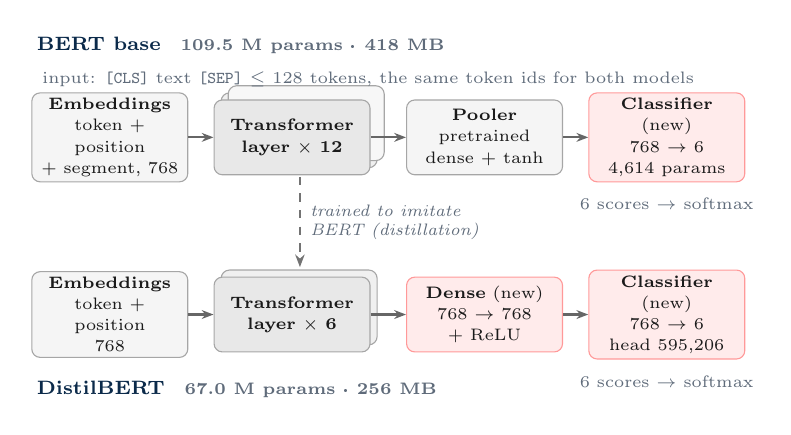
\begin{tikzpicture}[
  pre/.style={draw=black!35,fill=prec,rounded corners=3pt,align=center,font=\fontsize{6.4}{7.6}\selectfont,text=ink,text width=1.84cm,minimum height=0.95cm,inner sep=2pt},
  new/.style={pre,fill=newc,draw=red!40},
  lay/.style={pre,fill=black!9},
  ar/.style={-{Stealth[length=1.5mm]},thick,black!60},
  nm/.style={font=\scriptsize\bfseries,anchor=west}]
  % BERT row
  \node[nm,text=navy] at (-0.05,1.17) {BERT base {\fontsize{6}{7}\selectfont\color{muted}\enspace 109.5 M params \textperiodcentered{} 418 MB}};
  \node[pre] (be) at (1.0,0) {{\sbf Embeddings}\\token + position\\+ segment, 768};
  \node[lay,right=0.32cm of be] (bl) {{\sbf Transformer\\layer $\times$ 12}};
  \begin{scope}[on background layer]
    \node[lay,fill=black!6] at ($(bl)+(0.09,0.09)$) {};
    \node[lay,fill=black!3] at ($(bl)+(0.18,0.18)$) {};
  \end{scope}
  \node[pre,right=0.45cm of bl] (bp) {{\sbf Pooler}\\pretrained\\dense + tanh};
  \node[new,right=0.32cm of bp] (bc) {{\sbf Classifier} (new)\\768 $\rightarrow$ 6\\4,614 params};
  \draw[ar](be)--(bl); \draw[ar](bl)--(bp); \draw[ar](bp)--(bc);
  % DistilBERT row
  \node[nm,text=navy] at (-0.05,-3.2) {DistilBERT {\fontsize{6}{7}\selectfont\color{muted}\enspace 67.0 M params \textperiodcentered{} 256 MB}};
  \node[pre] (de) at (1.0,-2.25) {{\sbf Embeddings}\\token + position\\768};
  \node[lay,right=0.32cm of de] (dl) {{\sbf Transformer\\layer $\times$ 6}};
  \begin{scope}[on background layer]
    \node[lay,fill=black!6] at ($(dl)+(0.09,0.09)$) {};
  \end{scope}
  \node[new,right=0.45cm of dl] (dp) {{\sbf Dense} (new)\\768 $\rightarrow$ 768\\+ ReLU};
  \node[new,right=0.32cm of dp] (dc) {{\sbf Classifier} (new)\\768 $\rightarrow$ 6\\head 595,206};
  \draw[ar](de)--(dl); \draw[ar](dl)--(dp); \draw[ar](dp)--(dc);
  % distillation
  \draw[-{Stealth[length=1.6mm]},thick,dashed,black!55] ($(bl.south)+(0.1,-0.02)$) -- node[right,font=\fontsize{6}{7}\selectfont\itshape,text=muted,align=left]{trained to imitate\\BERT (distillation)} ($(dl.north)+(0.1,0.12)$);
  % input / output
  \node[font=\fontsize{6}{7}\selectfont,text=muted,anchor=west] at (0.02,0.74) {input: \texttt{[CLS]} text \texttt{[SEP]} $\le$ 128 tokens, the same token ids for both models};
    \node[font=\fontsize{6}{7}\selectfont,text=muted,anchor=north] at ($(bc.south)+(0,-0.08)$) {6 scores $\rightarrow$ softmax};
  \node[font=\fontsize{6}{7}\selectfont,text=muted,anchor=north] at ($(dc.south)+(0,-0.08)$) {6 scores $\rightarrow$ softmax};
\end{tikzpicture}
\vskip6pt
\raggedright
{\scriptsize\tikz[baseline=-0.6ex]\fill[black!9,draw=black!35](0,0)rectangle(0.3,0.18); \mut{pretrained, fine-tuned} \quad
 \tikz[baseline=-0.6ex]\fill[newc,draw=red!40](0,0)rectangle(0.3,0.18); \mut{new, random start}\par\vskip2pt
 \mut{Full fine-tuning updates every weight; the frozen variant trains the head only.}}
\column{0.28\textwidth}
\centering
\begin{tcolorbox}[enhanced,colback=white,colframe=linec,boxrule=0.4pt,arc=1pt,left=4pt,right=4pt,top=4pt,bottom=4pt,boxsep=0pt]
\centering{\fontsize{7.5}{9}\eb\color{navy}One Transformer layer}\par\vskip3pt
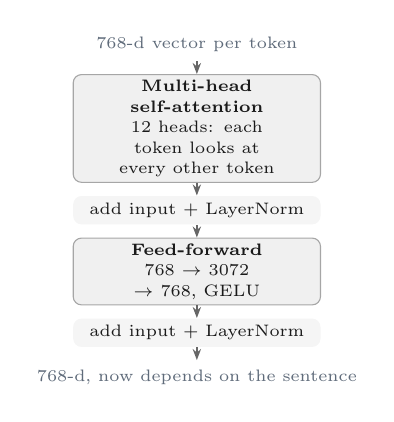
\begin{tikzpicture}[
  sb/.style={draw=black!35,rounded corners=3pt,align=center,font=\fontsize{6.2}{7.4}\selectfont,text=ink,text width=3.0cm,minimum height=0.6cm,inner sep=2pt},
  nb/.style={sb,fill=black!4,draw=none,minimum height=0.36cm},
  ar/.style={-{Stealth[length=1.4mm]},thick,black!60}, node distance=0.16cm]
  \node[font=\fontsize{6}{7}\selectfont,text=muted] (in) {768-d vector per token};
  \node[sb,fill=black!6,below=of in] (m) {{\sbf Multi-head self-attention}\\12 heads: each token looks at\\every other token};
  \node[nb,below=of m] (n1) {add input + LayerNorm};
  \node[sb,fill=black!6,below=of n1] (f) {{\sbf Feed-forward}\\768 $\rightarrow$ 3072 $\rightarrow$ 768, GELU};
  \node[nb,below=of f] (n2) {add input + LayerNorm};
  \node[font=\fontsize{6}{7}\selectfont,text=muted,below=of n2] (out) {768-d, now depends on the sentence};
  \draw[ar](in)--(m); \draw[ar](m)--(n1); \draw[ar](n1)--(f); \draw[ar](f)--(n2); \draw[ar](n2)--(out);
\end{tikzpicture}
\end{tcolorbox}
\end{columns}
\end{frame}

% ---------------------------------------------------------------------
\begin{frame}{Training setup}
\vskip2pt
\begin{columns}[T,onlytextwidth]
\column{0.6\textwidth}
\begin{card}
  \ctitle{Transformers (DistilBERT, BERT, frozen variant)}
  {\scriptsize\renewcommand{\arraystretch}{1.12}
  \begin{tabularx}{\linewidth}{@{}K{2.0cm}Y@{}}
    Loss & cross-entropy with class weights \mut{(love 2.07, surprise 4.71, joy 0.50)}\\
    Optimiser & AdamW, weight decay 0.01, gradient clip 1.0\\
    Learning rate & encoder $2\times10^{-5}$ \textperiodcentered{} head $1\times10^{-4}$\\
    Schedule & warmup 10\% (298 steps), then linear decay to 0\\
    Batch \textperiodcentered{} epochs & 16 \textperiodcentered{} 3 (2,988 steps); max 128 tokens, per-batch padding\\
    Checkpoint & the epoch with the best validation Macro-F1\\
    Seeds & 42, 43, 44 \mut{(42 = main run)}\\
  \end{tabularx}}
\end{card}
\column{0.37\textwidth}
\begin{card}
  \ctitle{Baseline}
  {\scriptsize\renewcommand{\arraystretch}{1.22}
  \begin{tabularx}{\linewidth}{@{}K{1.45cm}Y@{}}
    Features & TF-IDF, 1--2-grams, min\_df 2, max\_df 0.9\\
    Classifier & logistic regression, $C=1$, L-BFGS\\
    Weights & balanced \mut{(chosen in E4)}\\
    Text & aggressive \mut{(chosen in E3)}\\
  \end{tabularx}}
\end{card}
\vskip4pt
\begin{softcard}
  {\scriptsize No hyperparameter search: common starting values, the same for every run.}
\end{softcard}
\end{columns}
\vskip6pt
\begin{card}[top=3pt,bottom=3pt]
  {\scriptsize\sbf\color{navy}Colab T4, FP32 \textperiodcentered{} Python 3.13 \textperiodcentered{} PyTorch 2.14.1 \textperiodcentered{} transformers 5.22.1 \textperiodcentered{} scikit-learn 1.6.1 \textperiodcentered{} W\&B logs}
\end{card}
\end{frame}

% =====================================================================
\section{Results}
% =====================================================================
\begin{frame}{Final choice: DistilBERT, full fine-tune}
\vskip2pt
\begin{columns}[T,onlytextwidth]
\column{0.6\textwidth}
\begin{card}
  {\scriptsize\renewcommand{\arraystretch}{1.3}\setlength{\tabcolsep}{4pt}
  \begin{tabularx}{\linewidth}{@{}Y@{\hspace{3pt}}ccc@{}}
    \toprule
    \thd{Model} & \thd{Val Macro-F1} & \thd{Test Macro-F1} & \thd{Test Acc}\\
    & \mut{3 seeds, decides} & \mut{once, after} & \\
    \midrule
    \mut{Majority (joy)} & \mut{0.0868} & \mut{0.0860} & \mut{0.3475}\\
    \mdot{frozenc}\ Frozen DistilBERT & 0.4191 {\tiny\mut{$\pm$0.0061}} & 0.4199 & 0.5010\\
    \mdot{basec}\ TF-IDF + LR & 0.8758 & 0.8548 & 0.8905\\
    \hl \mdot{distilc}\ {\sbf DistilBERT full} & {\sbf 0.9155} {\tiny\mut{$\pm$0.0020}} & {\sbf 0.8902} & {\sbf 0.9270}\\
    \mdot{bertc}\ BERT full & 0.9163 {\tiny\mut{$\pm$0.0032}} & 0.8881 & 0.9280\\
    \bottomrule
  \end{tabularx}}
  \vskip3pt
  {\fontsize{6}{7.5}\selectfont\mut{Test columns = seed-42 run. The choice was fixed on validation before any test result.}}
\end{card}
\vskip4pt
\begin{softcard}
  {\scriptsize{\sbf Where context helps} \mut{(test text, true label: fear)}\par\vskip2pt
  \quot{i was feeling pretty anxious all day {\sbf but} my first day at work was a very good day and that helped a lot}\par\vskip2pt
  DistilBERT: fear \yes \qquad TF-IDF baseline: joy \no}
\end{softcard}
\column{0.375\textwidth}
\begin{card}
  \ctitle{Why DistilBERT?}
  {\footnotesize
  \begin{tabularx}{\linewidth}{@{}c@{\hspace{5pt}}Y@{}}
    \yes & {\sbf Beats the baseline:} +0.035 test Macro-F1, better on all 6 classes\\[3pt]
    {\sbf\color{accent}=} & {\sbf Ties with BERT:} gap +0.0008 is below the seed noise 0.0032 $\rightarrow$ keep the smaller model\\[3pt]
    \no & {\sbf Frozen encoder fails:} $-$0.50, even below the baseline\\
  \end{tabularx}}
\end{card}
\vskip4pt
\begin{softcard}
  {\scriptsize 124 test texts only DistilBERT gets right vs.\ 51 only the baseline (McNemar $p\approx3\times10^{-8}$)}
\end{softcard}
\end{columns}
\end{frame}

% ---------------------------------------------------------------------
\begin{frame}{How we decide: the gap vs.\ the seed noise}
\vskip2pt
\begin{columns}[T,onlytextwidth]
\column{0.485\textwidth}
\begin{card}
  \tagc{accent}{RULE A \textperiodcentered{} REAL DIFFERENCE (E1)}\par\vskip3pt
  {\footnotesize A wins on {\sbf all 3 seeds} and the mean gap is {\sbf $>$ 2 $\times$ the larger seed std}}\par\vskip4pt
  \centering
  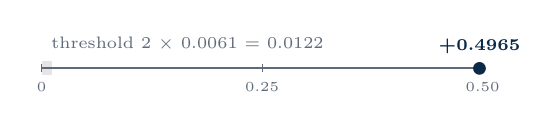
\begin{tikzpicture}[x=11.2cm]
    \fill[black!10] (0,-0.09) rectangle (0.0122,0.09);
    \draw[muted,thick] (0,0)--(0.5,0);
    \foreach \v/\l in {0/0,0.25/0.25,0.5/0.50} {\draw[muted](\v,-0.05)--(\v,0.05); \node[font=\fontsize{5.5}{6}\selectfont,text=muted,below] at (\v,-0.05){\l};}
    \fill[navy] (0.4965,0) circle (2.3pt);
    \node[font=\fontsize{6}{7}\selectfont\sbf,text=navy,above] at (0.4965,0.06) {+0.4965};
    \node[font=\fontsize{6}{7}\selectfont,text=muted,above,align=left,anchor=south west] at (0,0.1) {threshold 2 $\times$ 0.0061 = 0.0122};
  \end{tikzpicture}\par\vskip1pt
  \raggedright{\scriptsize full $-$ frozen: about {\sbf 40$\times$} the threshold $\rightarrow$ real gap}
\end{card}
\column{0.485\textwidth}
\begin{card}
  \tagc{accentB}{RULE B \textperiodcentered{} TIE (E2, FINAL CHOICE)}\par\vskip3pt
  {\footnotesize $|$mean gap$|$ {\sbf $<$ the larger seed std} $\rightarrow$ tie $\rightarrow$ keep the {\sbf smaller} model}\par\vskip4pt
  \centering
  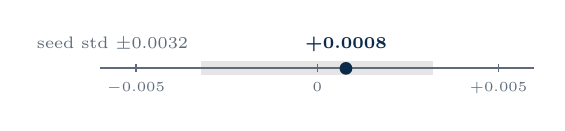
\begin{tikzpicture}[x=460cm]
    \fill[black!10] (-0.0032,-0.09) rectangle (0.0032,0.09);
    \draw[muted,thick] (-0.006,0)--(0.006,0);
    \foreach \v/\l in {-0.005/$-$0.005,0/0,0.005/+0.005} {\draw[muted](\v,-0.05)--(\v,0.05); \node[font=\fontsize{5.5}{6}\selectfont,text=muted,below] at (\v,-0.05){\l};}
    \fill[navy] (0.0008,0) circle (2.3pt);
    \node[font=\fontsize{6}{7}\selectfont\sbf,text=navy,above] at (0.0008,0.08) {+0.0008};
    \node[font=\fontsize{6}{7}\selectfont,text=muted,anchor=south east] at (-0.0033,0.1) {seed std $\pm$0.0032};
  \end{tikzpicture}\par\vskip1pt
  \raggedright{\scriptsize BERT $-$ DistilBERT: inside the noise band $\rightarrow$ tie}
\end{card}
\end{columns}
\vskip6pt
{\footnotesize\bfseries\color{navy}Why this heuristic?}\par\vskip3pt
\begin{tcbraster}[raster columns=4,raster equal height,raster column skip=5pt]
  \begin{softcard}{\scriptsize{\bfseries\color{navy}1}\ \ Written down {\sbf before} the runs, as the handbook asks}\end{softcard}
  \begin{softcard}{\scriptsize{\bfseries\color{navy}2}\ \ Seed std = the noise from changing {\sbf only the seed}}\end{softcard}
  \begin{softcard}{\scriptsize{\bfseries\color{navy}3}\ \ $\times$2 ($\approx$95\% idea) + win on every seed = {\sbf conservative}}\end{softcard}
  \begin{softcard}{\scriptsize{\bfseries\color{navy}4}\ \ 3 seeds: formal tests are weak, so a {\sbf simple rule} + McNemar per text}\end{softcard}
\end{tcbraster}
\end{frame}

% =====================================================================
\section{Controlled experiments}
% =====================================================================
\begin{frame}{E1 (main): frozen encoder vs.\ full fine-tune}
\vskip2pt
\begin{columns}[T,onlytextwidth]
\column{0.5\textwidth}
\begin{card}
  {\scriptsize\renewcommand{\arraystretch}{1.25}
  \begin{tabularx}{\linewidth}{@{}K{1.55cm}Y@{}}
    Hypothesis & pretrained features are not tuned to emotions $\rightarrow$ frozen is clearly worse, but trains faster\\
    Changed & encoder frozen (595,206 trainable, 0.89\%) vs.\ all 66,958,086 trained\\
    Fixed & data, text, token ids, batch order, seeds, head LR, schedule, 3 epochs, class weights\\
    Metric & val Macro-F1, mean $\pm$ std over 3 seeds\\
    Criterion & (1) real gap = rule A \quad (2) good enough = drop $\le$ 0.02\\
  \end{tabularx}}
\end{card}
\column{0.475\textwidth}
\begin{tcbraster}[raster columns=2,raster equal height,raster column skip=5pt]
  \kpi[frozenc]{0.4191}{frozen, val \textperiodcentered{} $\pm$ 0.0061}
  \kpi[distilc]{0.9155}{full, val \textperiodcentered{} $\pm$ 0.0020}
\end{tcbraster}
\vskip4pt
\begin{card}
  {\scriptsize\renewcommand{\arraystretch}{1.3}
  \begin{tabularx}{\linewidth}{@{}c@{\hspace{5pt}}Y@{}}
    \yes & (1) full wins on 3/3 seeds; gap 0.4965 $\gg$ 0.0122\\
    \no & (2) drop 0.50 $\gg$ 0.02 $\rightarrow$ {\sbf frozen excluded}\\
    \yes & test check: +0.4651, 3/3 seeds\\
  \end{tabularx}}
\end{card}
\end{columns}
\vskip6pt
\begin{tcbraster}[raster columns=3,raster equal height,raster column skip=5pt]
  \begin{softcard}{\scriptsize{\sbf Underfits:} train = val loss 1.425, still falling when the LR reaches 0}\end{softcard}
  \begin{softcard}{\scriptsize{\sbf Cost:} 29\% of the training time, but {\sbf not} faster at inference}\end{softcard}
  \begin{softcard}{\scriptsize{\sbf Limit:} one recipe only (same head LR, 3 epochs)}\end{softcard}
\end{tcbraster}
\end{frame}

% ---------------------------------------------------------------------
\begin{frame}{E2: does a bigger encoder help?}
\vskip2pt
\begin{columns}[T,onlytextwidth]
\column{0.46\textwidth}
\begin{card}
  {\scriptsize\renewcommand{\arraystretch}{1.25}
  \begin{tabularx}{\linewidth}{@{}K{1.55cm}Y@{}}
    Hypothesis & the deeper BERT may gain a little at about twice the cost; is the gain above seed noise?\\
    Changed & pretrained model: BERT vs.\ DistilBERT\\
    Fixed & same token ids, data, recipe, batch order, seeds\\
    Metric & val Macro-F1, mean $\pm$ std over 3 seeds, and seed by seed\\
    Criterion & rule B: $|$gap$|$ $<$ seed std $\rightarrow$ tie $\rightarrow$ smaller model\\
  \end{tabularx}}
\end{card}
\vskip4pt
\begin{softcard}
  {\scriptsize{\sbf Limit:} the swap bundles depth, BERT's pooler and distillation, so it shows {\sbf whether} BERT differs, not {\sbf why}.}
\end{softcard}
\column{0.515\textwidth}
\begin{card}
  \ctitle{BERT $-$ DistilBERT, Macro-F1}
  {\scriptsize\renewcommand{\arraystretch}{1.25}
  \begin{tabularx}{\linewidth}{@{}Ycc@{}}
    \toprule
    \thd{Seed} & \thd{Validation} & \thd{Test}\\
    \midrule
    42 & +0.0051 & $-$0.0021\\
    43 & $-$0.0033 & +0.0023\\
    44 & +0.0005 & +0.0047\\
    \hl {\sbf Mean} & {\sbf +0.0008} \mut{$<$ 0.0032} & {\sbf +0.0016} \mut{$<$ 0.0038}\\
    \bottomrule
  \end{tabularx}}
  \vskip4pt
  {\footnotesize\bfseries\color{navy}Tie on both splits $\rightarrow$ keep DistilBERT}
\end{card}
\vskip4pt
\begin{tcbraster}[raster columns=2,raster equal height,raster column skip=5pt]
  \begin{softcard}{\scriptsize{\sbf McNemar (test):} 62 vs.\ 60 texts, $p\approx0.93$}\end{softcard}
  \begin{softcard}{\scriptsize{\sbf Cost:} $\times$1.64 params, $\times$1.89 train, $\times$2.00 CPU latency}\end{softcard}
\end{tcbraster}
\end{columns}
\end{frame}

% ---------------------------------------------------------------------
\begin{frame}{E3 and E4: two cheap fixes for the baseline}
\vskip2pt
\begin{tcbraster}[raster columns=2,raster equal height,raster column skip=6pt]
\begin{card}
  \tagc{basec}{E3}\ {\eb\color{navy}Stopwords removed vs.\ kept}\par\vskip3pt
  {\scriptsize\renewcommand{\arraystretch}{1.1}
  \begin{tabularx}{\linewidth}{@{}K{1.45cm}Y@{}}
    Hypothesis & the signal is in emotion words, so little change\\
    Changed & text: aggressive vs.\ minimal\\
    Fixed & TF-IDF settings, $C=1$, class weights\\
    Metric & val Macro-F1\\
    Rule & higher wins; a tie keeps the minimal text\\
  \end{tabularx}}
  \vskip3pt
  {\fontsize{13}{15}\bfseries\color{navy}+0.0269}\ {\scriptsize\mut{val (0.8758 vs.\ 0.8489) \textperiodcentered{} test +0.0183}}\par\vskip2pt
  {\scriptsize F1 up on all 6 classes with half the n-grams; negated texts: accuracy 0.846 $\rightarrow$ 0.891\par\vskip2pt
  \no\ {\sbf Rejected:} \textit{not} now sits next to the emotion word $\rightarrow$ bigram \quot{not happy}}
\end{card}
\begin{card}
  \tagc{basec}{E4 \textperiodcentered{} ABLATION}\ {\eb\color{navy}Class weights on vs.\ off}\par\vskip3pt
  {\scriptsize\renewcommand{\arraystretch}{1.1}
  \begin{tabularx}{\linewidth}{@{}K{1.45cm}Y@{}}
    Hypothesis & small classes gain recall, lose some precision\\
    Changed & class weights: balanced vs.\ none\\
    Fixed & minimal text, TF-IDF settings, $C=1$\\
    Metric & val Macro-F1; per-class P / R / F1\\
    Rule & higher wins; a tie keeps no weights\\
  \end{tabularx}}
  \vskip3pt
  {\fontsize{13}{15}\bfseries\color{navy}+0.096}\ {\scriptsize\mut{val (0.8489 vs.\ 0.7527) \textperiodcentered{} test +0.108}}\par\vskip2pt
  {\scriptsize surprise recall 0.40 $\rightarrow$ 0.81, precision 0.89 $\rightarrow$ 0.73; F1 up on all 6 classes\par\vskip2pt
  \yes\ {\sbf Supported:} class weights used for every later model}
\end{card}
\end{tcbraster}
\vskip4pt
\begin{banner}
  Together they lift the baseline from 0.7289 to 0.8548 test Macro-F1.
\end{banner}
\end{frame}

% =====================================================================
\section{Compute cost}
% =====================================================================
\begin{frame}{Compute cost}
\vskip2pt
\begin{card}[left=5pt,right=5pt]
  {\scriptsize\renewcommand{\arraystretch}{1.18}\setlength{\tabcolsep}{4pt}
  \begin{tabularx}{\linewidth}{@{}Yrrrrrrc@{}}
    \toprule
    & & & & \thd{Batched} & \multicolumn{2}{c}{\thd{One text (ms)}} & \\
    \cmidrule(lr){6-7}
    \thd{Model} & \thd{Trainable params} & \thd{Size} & \thd{Train time} & \thd{ms / text} & \thd{CPU} & \thd{GPU} & \thd{Test Macro-F1}\\
    \midrule
    \mdot{basec}\ TF-IDF + LR & 102,426 & 1.17 MB & 5.3 s \mut{CPU} & 0.015 \mut{CPU} & 1.32 & -- & 0.8548\\
    \mdot{distilc}\ DistilBERT, full & 66,958,086 & 256 MB & 276.9 $\pm$ 10.5 s & 1.63 & 59.6 & 5.92 & 0.8861\\
    \mdot{frozenc}\ DistilBERT, frozen & 595,206 & 256 MB & 81.4 $\pm$ 0.4 s & 1.59 & 60.9 & 4.71 & 0.4210\\
    \rowcolor{black!7}\mdot{bertc}\ {\sbf BERT, full} & {\sbf 109,486,854} & {\sbf 418 MB} & {\sbf 524.7 $\pm$ 0.5 s} & {\sbf 3.16} & {\sbf 119.2} & {\sbf 8.79} & 0.8878\\
    \bottomrule
  \end{tabularx}}
  \vskip2pt
  {\fontsize{6}{7.5}\selectfont\mut{Transformers on a T4 GPU. Time: median of 5 repeats after a warm-up; one-text latency on the same CPU (1 thread). Train time and test Macro-F1: mean over 3 seeds.}}
\end{card}
\vskip5pt
\begin{tcbraster}[raster columns=3,raster equal height,raster column skip=5pt]
  \begin{card}
    \ctitle{BERT costs the most}
    {\scriptsize $\times$1.64 params, $\times$1.89 train time, $\times$2.00 CPU latency of DistilBERT, for {\sbf +0.0016} F1}
  \end{card}
  \begin{card}
    \ctitle{Baseline is the cheapest}
    {\scriptsize 45$\times$ faster on CPU, 219$\times$ smaller than DistilBERT, for {\sbf $-$0.031} F1}
  \end{card}
  \begin{card}
    \ctitle{Freezing saves training only}
    {\scriptsize 29\% of the training time; same forward pass, same inference cost}
  \end{card}
\end{tcbraster}
\end{frame}

% =====================================================================
\section{Error analysis}
% =====================================================================
\begin{frame}{Where do the 146 errors go?}
\vskip2pt
\begin{columns}[T,onlytextwidth]
\column{0.42\textwidth}
\begin{card}
  \ctitle{How the pairs were chosen}
  \begin{enumerate}\setlength{\itemsep}{2pt}\scriptsize
    \item Count every true $\rightarrow$ predicted pair \mut{(19 of the 30 possible pairs occur)}
    \item Rank by count: top 3 = {\sbf 45\%} of the errors, top 10 = {\sbf 84\%}
    \item Merge a pair with its reverse and its neighbours: {\sbf 3 groups}, one cause each
    \item Also check the share of the class: surprise $\rightarrow$ fear is {\sbf 15\%} of all surprise texts
  \end{enumerate}
\end{card}
\vskip4pt
\begin{softcard}
  {\scriptsize\sbf Every pair links two close emotions; none links opposites like joy $\leftrightarrow$ anger.}
\end{softcard}
\column{0.555\textwidth}
\begin{card}[left=5pt,right=5pt]
  {\scriptsize\renewcommand{\arraystretch}{1.08}\setlength{\tabcolsep}{4pt}
  \begin{tabularx}{\linewidth}{@{}Ycccrl@{}}
    \toprule
    \thd{True $\rightarrow$ predicted} & \mdot{distilc} & \mdot{basec} & \mdot{bertc} & \thd{\% class} & \\
    \midrule
    \hl joy $\rightarrow$ love & {\sbf 42} & 58 & 20 & 6.0 & \tagc{accent}{G1}\\
    anger $\rightarrow$ sadness & 12 & 8 & 17 & 4.4 & \tagc{frozenc}{G2}\\
    anger $\rightarrow$ fear & 12 & 7 & 7 & 4.4 & \tagc{frozenc}{G2}\\
    fear $\rightarrow$ surprise & 11 & 19 & 26 & 4.9 & \tagc{bertc}{G3}\\
    sadness $\rightarrow$ anger & 11 & 23 & 5 & 1.9 & \tagc{frozenc}{G2}\\
    \hl surprise $\rightarrow$ fear & 10 & 2 & 0 & {\sbf 15.2} & \tagc{bertc}{G3}\\
    joy $\rightarrow$ surprise & 7 & 11 & 7 & 1.0 & \tagc{basec}{other}\\
    love $\rightarrow$ joy & 6 & 8 & 28 & 3.8 & \tagc{accent}{G1}\\
    sadness $\rightarrow$ fear & 6 & 8 & 2 & 1.0 & \tagc{frozenc}{G2}\\
    fear $\rightarrow$ sadness & 6 & 8 & 5 & 2.7 & \tagc{frozenc}{G2}\\
    \bottomrule
  \end{tabularx}}
  \vskip2pt
  {\fontsize{6}{7.5}\selectfont\mut{Test errors: \mdot{distilc} DistilBERT 146, \mdot{basec} baseline 219, \mdot{bertc} BERT 144. \% class = share of the true class (DistilBERT).}}
\end{card}
\end{columns}
\end{frame}

% ---------------------------------------------------------------------
\begin{frame}{Three error groups, and a label-noise signal}
\vskip2pt
\begin{card}[left=5pt,right=5pt]
  {\scriptsize\renewcommand{\arraystretch}{1.12}\setlength{\tabcolsep}{4pt}
  \begin{tabularx}{\linewidth}{@{}>{\raggedright\arraybackslash}p{3.1cm}ccc>{\raggedright\arraybackslash}p{4.0cm}Y@{}}
    \toprule
    \thd{Group} & \mdot{distilc} & \mdot{basec} & \mdot{bertc} & \thd{Likely cause} & \thd{Possible fix}\\
    \midrule
    \tagc{accent}{G1} joy $\leftrightarrow$ love & 48 & 66 & 48 & shared words; love weight 2.07 vs.\ joy 0.50 & more love data; per-class thresholds\\
    \tagc{frozenc}{G2} sadness/anger/fear & 51 & 61 & 45 & one negative word fits several emotions & multi-label; use more context\\
    \tagc{bertc}{G3} fear $\leftrightarrow$ surprise & 21 & 21 & 26 & smallest class; \textit{overwhelmed}, \textit{shocked} & more surprise data; threshold\\
    \tagc{basec}{other} scattered & 26 & {\sbf 71} & 25 & keyword errors of the baseline & --\\
    \bottomrule
  \end{tabularx}}
  \vskip2pt
  {\fontsize{6}{7.5}\selectfont\mut{G1: \quot{\ldots feel his force supporting me as i teach} joy$\rightarrow$love \quad G2: \quot{when i learnt that my best friend had failed the exams} anger$\rightarrow$sadness \quad G3: \quot{i started to feel so overwhelmed} fear$\rightarrow$surprise}}
\end{card}
\vskip5pt
\begin{tcbraster}[raster columns=3,raster equal height,raster column skip=5pt,raster force size=false]
  \begin{card}[add to width=-0.7cm]
    {\fontsize{14}{16}\bfseries\color{navy}50}\enspace{\scriptsize test texts: all 3 models give the {\sbf same wrong} label \mut{(34\% of DistilBERT errors)}}
  \end{card}
  \begin{card}[add to width=-0.7cm]
    {\fontsize{14}{16}\bfseries\color{navy}9 / 9}\enspace{\scriptsize disputed test texts: the error is the label of the removed copy}
  \end{card}
  \begin{banner}[add to width=1.4cm,fontupper=\scriptsize\bfseries]
    Transformers remove the scattered errors (71 $\rightarrow$ 26), not the close-emotion boundaries: the limit is the labels, not model size.
  \end{banner}
\end{tcbraster}
\end{frame}

% =====================================================================
\section{Live demo}
% =====================================================================
\begin{frame}{Live demo: try it in your browser}
\vskip2pt
\begin{columns}[T,onlytextwidth]
\column{0.47\textwidth}
\centering
\href{https://huggingface.co/spaces/TrieuVo/goat-a2-emotion-demo}{%
\begin{tcolorbox}[enhanced,colback=white,colframe=linec,boxrule=0.4pt,arc=1pt,left=2pt,right=2pt,top=2pt,bottom=2pt,boxsep=0pt,width=6.0cm]
  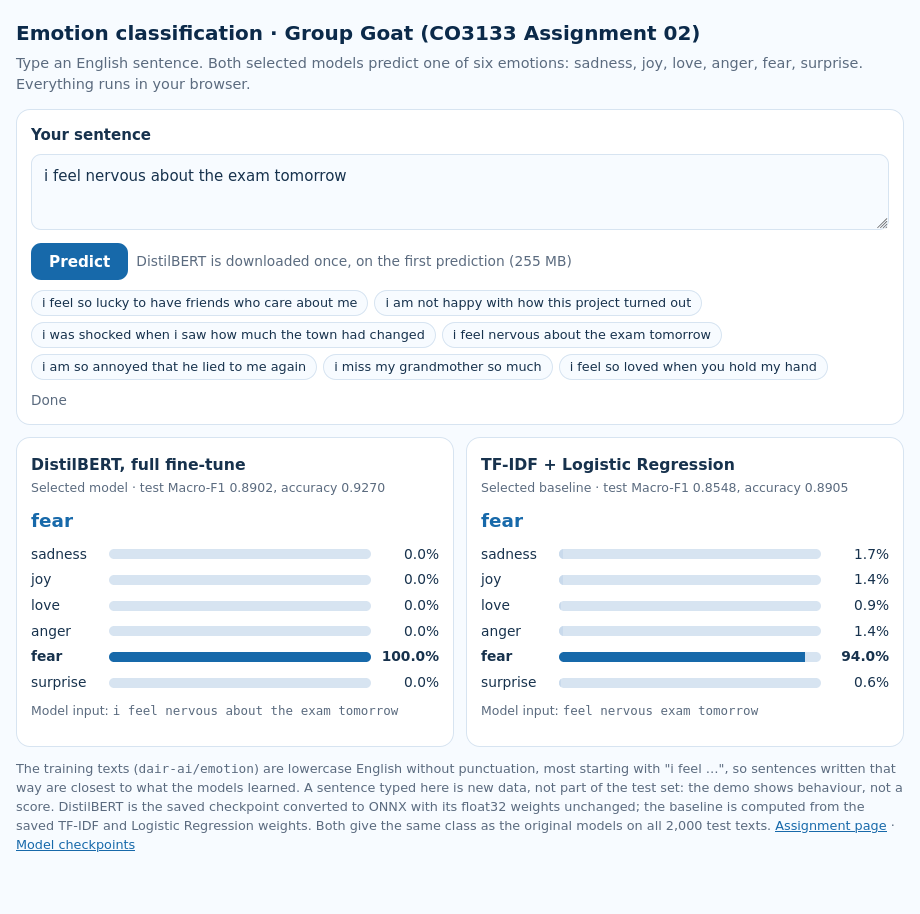
\includegraphics[width=\linewidth,trim=0 70 0 0,clip]{figures/demo_space.png}
\end{tcolorbox}}
\column{0.5\textwidth}
\begin{columns}[T,onlytextwidth]
\column{0.68\linewidth}
\vskip6pt
\href{https://huggingface.co/spaces/TrieuVo/goat-a2-emotion-demo}{%
\tikz\node[rectangle,draw=accent,inner xsep=8pt,inner ysep=4pt,font=\small\bfseries,text=accent]{Open the live demo $\nearrow$};}
\par\vskip4pt
{\fontsize{5.5}{6.5}\selectfont\mut{huggingface.co/spaces/TrieuVo/\\goat-a2-emotion-demo}}
\column{0.3\linewidth}
\raggedleft
\begin{tcolorbox}[enhanced,colback=white,colframe=linec,boxrule=0.4pt,arc=1pt,left=3pt,right=3pt,top=3pt,bottom=3pt,boxsep=0pt,width=1.75cm]
\centering\qrcode[height=1.4cm]{https://huggingface.co/spaces/TrieuVo/goat-a2-emotion-demo}
\end{tcolorbox}
\end{columns}
\vskip5pt
\begin{card}
  {\scriptsize
  \begin{itemize}\setlength{\itemsep}{3pt}
    \item Our {\sbf DistilBERT} and {\sbf TF-IDF baseline}, side by side
    \item Runs fully in the browser (ONNX + transformers.js), no server
    \item Same class as our checkpoints on all 2,000 test texts
  \end{itemize}}
\end{card}
\vskip5pt
{\footnotesize\bfseries\color{navy}Try}\par\vskip3pt
\chip{i feel nervous about the exam tomorrow}\ \chip{i miss my grandmother so much}\par\vskip3pt
\chip{i am not happy with how this project turned out}
\end{columns}
\end{frame}

% =====================================================================
\section{Conclusion}
% =====================================================================
\begin{frame}{Conclusion}
\vskip2pt
\begin{tcbraster}[raster columns=2,raster equal height,raster column skip=6pt,raster row skip=5pt]
  \begin{card}
    {\fontsize{14}{16}\bfseries\color{navy}0.8902 vs.\ 0.8548}\par\vskip2pt
    {\footnotesize{\sbf Fine-tuning beats TF-IDF}, on all 6 classes, most on long, negated and \quot{but} texts}
  \end{card}
  \begin{card}
    {\fontsize{14}{16}\bfseries\color{navy}+0.0016 for $\times$2 cost}\par\vskip2pt
    {\footnotesize{\sbf A bigger model does not help here:} BERT ties with DistilBERT}
  \end{card}
  \begin{card}
    {\fontsize{14}{16}\bfseries\color{navy}0.42}\par\vskip2pt
    {\footnotesize{\sbf The encoder must adapt:} frozen DistilBERT is worse than the baseline}
  \end{card}
  \begin{card}
    {\fontsize{14}{16}\bfseries\color{navy}0.7289 $\rightarrow$ 0.8548}\par\vskip2pt
    {\footnotesize{\sbf Cheap fixes matter:} class weights + stopword removal; still 45$\times$ faster on CPU}
  \end{card}
\end{tcbraster}
\vskip6pt
\begin{columns}[T,onlytextwidth]
\column{0.49\textwidth}
\begin{softcard}
  {\scriptsize{\sbf Limits:} noisy machine-generated labels \textperiodcentered{} no hyperparameter search \textperiodcentered{} only 3 seeds}
\end{softcard}
\column{0.49\textwidth}
\begin{softcard}
  {\scriptsize{\sbf Next:} per-class thresholds \textperiodcentered{} relabel doubtful texts \textperiodcentered{} multi-label targets}
\end{softcard}
\end{columns}
\end{frame}

% ---------------------------------------------------------------------
{\setbeamertemplate{frametitle}{}
\begin{frame}
\vskip1.0cm
\centering
{\Huge\bfseries\color{navy}Thank you}\par\vskip4pt
{\small\mut{Questions are welcome.}}\par\vskip14pt
\begin{tcbraster}[raster columns=3,raster equal height,raster column skip=6pt,raster width=0.92\textwidth,raster halign=center]
  \begin{card}\ctitle{Report page}{\scriptsize\href{https://volethanhtrieu.github.io/DL_Assignment-02/}{volethanhtrieu.github.io\\/DL\_Assignment-02}}\end{card}
  \begin{card}\ctitle{Code}{\scriptsize\href{https://github.com/volethanhtrieu/DL_Assignment-02}{github.com/volethanhtrieu\\/DL\_Assignment-02}}\end{card}
  \begin{card}\ctitle{Live demo}{\scriptsize\href{https://huggingface.co/spaces/TrieuVo/goat-a2-emotion-demo}{huggingface.co/spaces/TrieuVo\\/goat-a2-emotion-demo}}\end{card}
  \begin{card}\ctitle{Checkpoints}{\scriptsize\href{https://huggingface.co/TrieuVo/goat-a2-emotion}{huggingface.co/TrieuVo\\/goat-a2-emotion}}\end{card}
  \begin{card}\ctitle{Experiment logs}{\scriptsize\href{https://wandb.ai/trieu-vo1301-ho-chi-minh-city-university-of-technology/goat-a2-emotion}{W\&B project goat-a2-emotion}}\end{card}
  \begin{card}\ctitle{Presentation video}{\scriptsize\href{https://www.youtube.com/watch?v=ok-hF_vicjc}{youtube.com/watch\\?v=ok-hF\_vicjc}}\end{card}
\end{tcbraster}
\end{frame}}

% =====================================================================
%  BACKUP (not shown in the video; for questions)
% =====================================================================
\appendix
\backuptrue

\begin{frame}{Per-class F1 on test (seed-42 runs)}
\vskip2pt
\begin{card}
  {\scriptsize\renewcommand{\arraystretch}{1.3}
  \begin{tabularx}{\linewidth}{@{}Yrccccc@{}}
    \toprule
    \thd{Class} & \thd{Test texts} & \mdot{basec}\ \thd{Baseline} & \mdot{distilc}\ \thd{DistilBERT} & \mdot{bertc}\ \thd{BERT} & \mdot{frozenc}\ \thd{Frozen} & \thd{DistilBERT val}\\
    \midrule
    sadness & 581 & 0.9296 & 0.9612 & 0.9643 & 0.5299 & 0.9616\\
    joy & 695 & 0.9110 & 0.9504 & 0.9513 & 0.6492 & 0.9561\\
    love & 159 & 0.7925 & 0.8523 & 0.8452 & 0.3435 & 0.8853\\
    anger & 275 & 0.8917 & 0.9134 & 0.9202 & 0.4329 & 0.9375\\
    fear & 224 & 0.8631 & 0.8904 & 0.8825 & 0.4219 & 0.8929\\
    surprise & 66 & 0.7407 & 0.7737 & 0.7654 & 0.1421 & 0.8554\\
    \midrule
    \hl {\sbf Macro-F1} & 2,000 & 0.8548 & {\sbf 0.8902} & 0.8881 & 0.4199 & 0.9148\\
    \bottomrule
  \end{tabularx}}
  \vskip3pt
  {\fontsize{6}{7.5}\selectfont\mut{The val $\rightarrow$ test drop of the strong models comes mostly from surprise (DistilBERT $-$0.082, only 66 test texts) and love ($-$0.033).}}
\end{card}
\end{frame}

\begin{frame}{Training curves (seed-42 runs)}
\vskip2pt
\begin{card}[left=3pt,right=3pt,top=3pt,bottom=3pt]
  \centering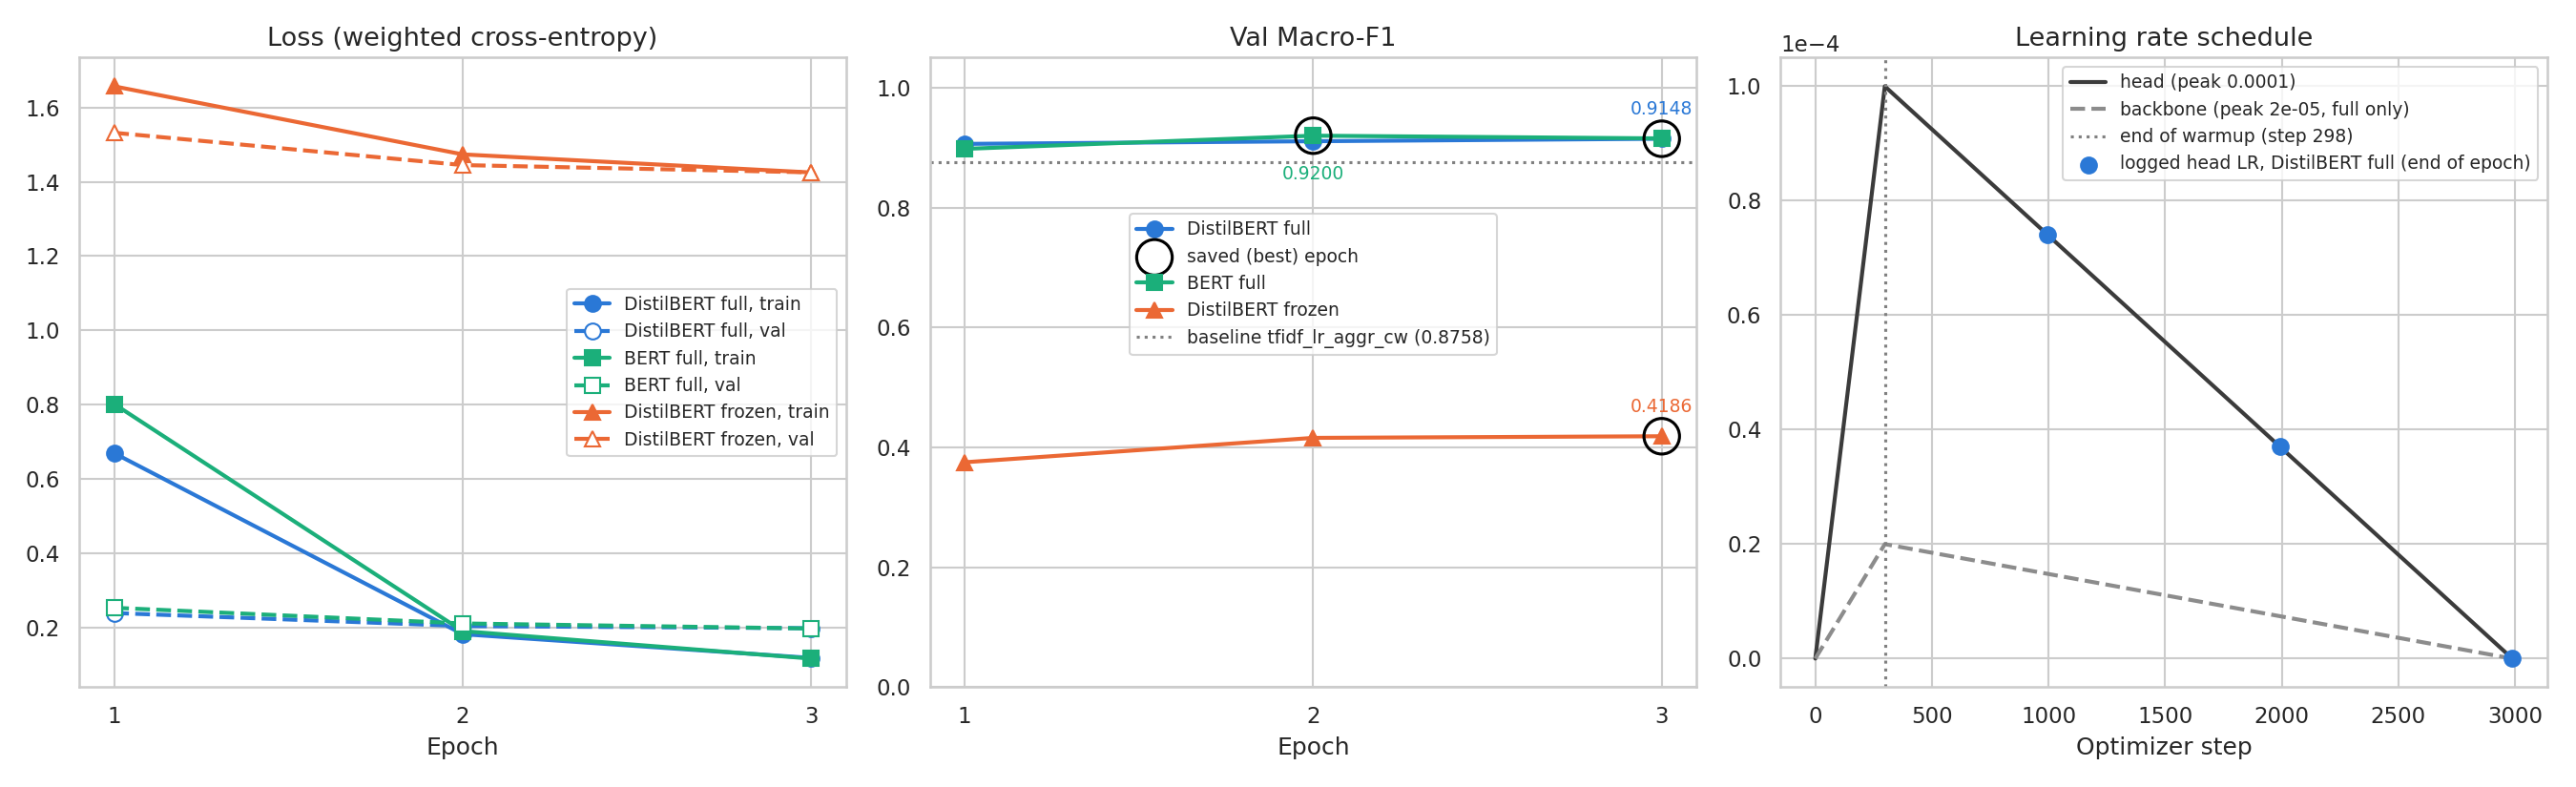
\includegraphics[width=\linewidth]{figures/a2_curves_final.png}
\end{card}
\vskip4pt
{\scriptsize\mut{Left: loss (solid = train, dashed = val). Middle: val Macro-F1, saved epoch circled, dotted line = baseline. Right: learning rate per step. Full runs converge in 3 epochs; frozen runs underfit.}}
\end{frame}

\begin{frame}{Confusion matrices on test (seed-42 runs)}
\vskip2pt
\begin{tcbraster}[raster columns=4,raster equal height,raster column skip=4pt]
  \begin{card}[left=2pt,right=2pt,top=2pt,bottom=3pt]\centering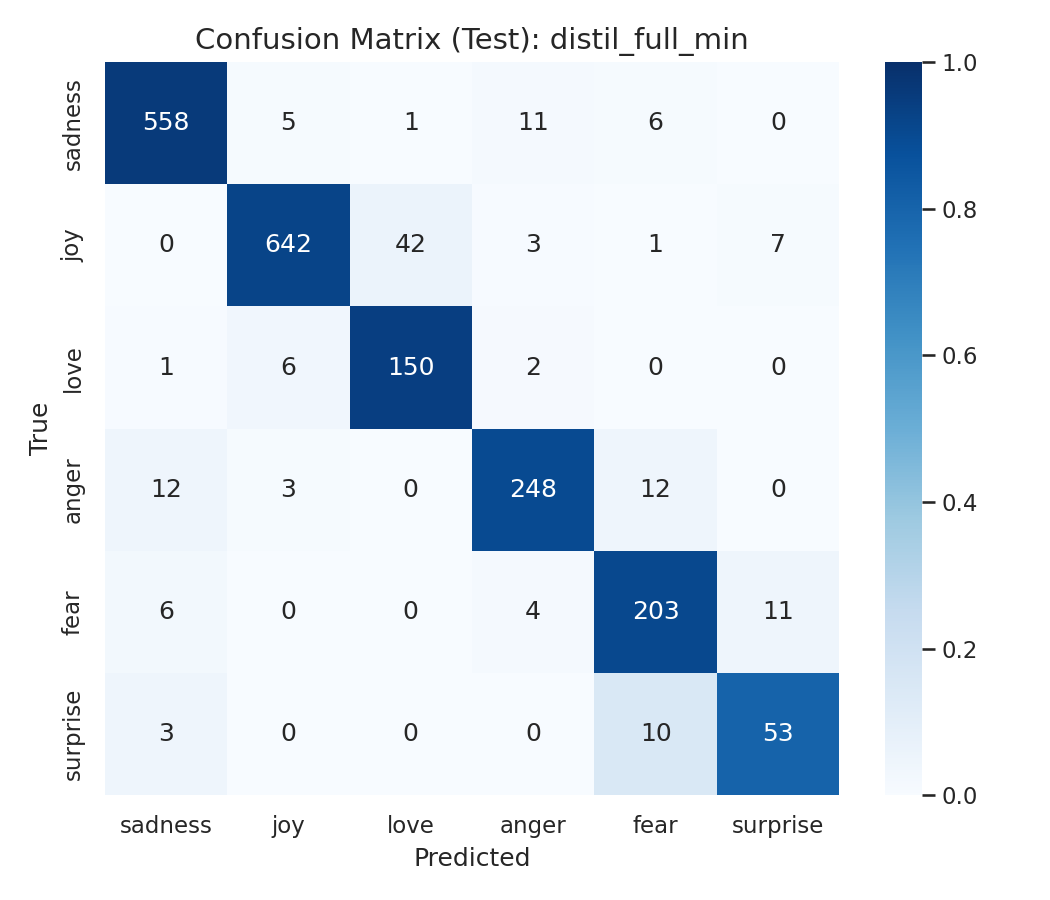
\includegraphics[width=\linewidth]{figures/a2_cm_test_distil_full_min.png}\par{\fontsize{6}{7}\sbf\selectfont DistilBERT \mut{0.8902}}\end{card}
  \begin{card}[left=2pt,right=2pt,top=2pt,bottom=3pt]\centering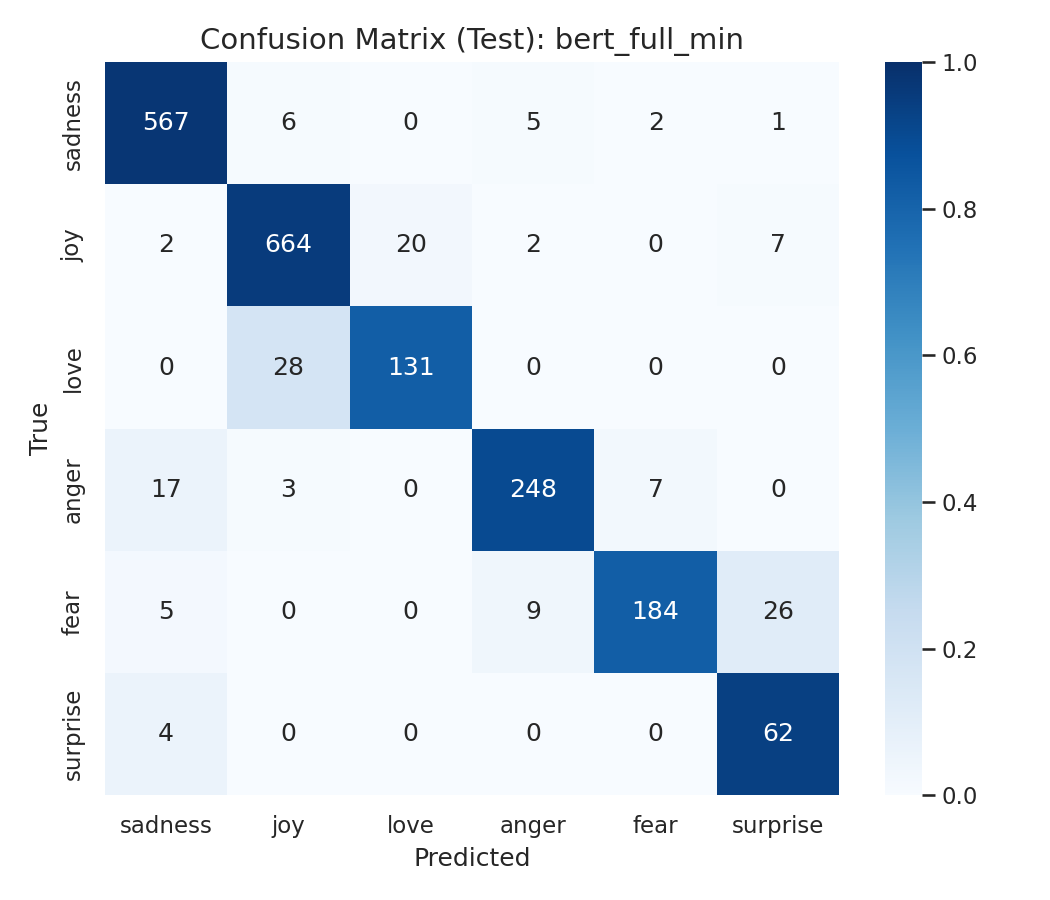
\includegraphics[width=\linewidth]{figures/a2_cm_test_bert_full_min.png}\par{\fontsize{6}{7}\sbf\selectfont BERT \mut{0.8881}}\end{card}
  \begin{card}[left=2pt,right=2pt,top=2pt,bottom=3pt]\centering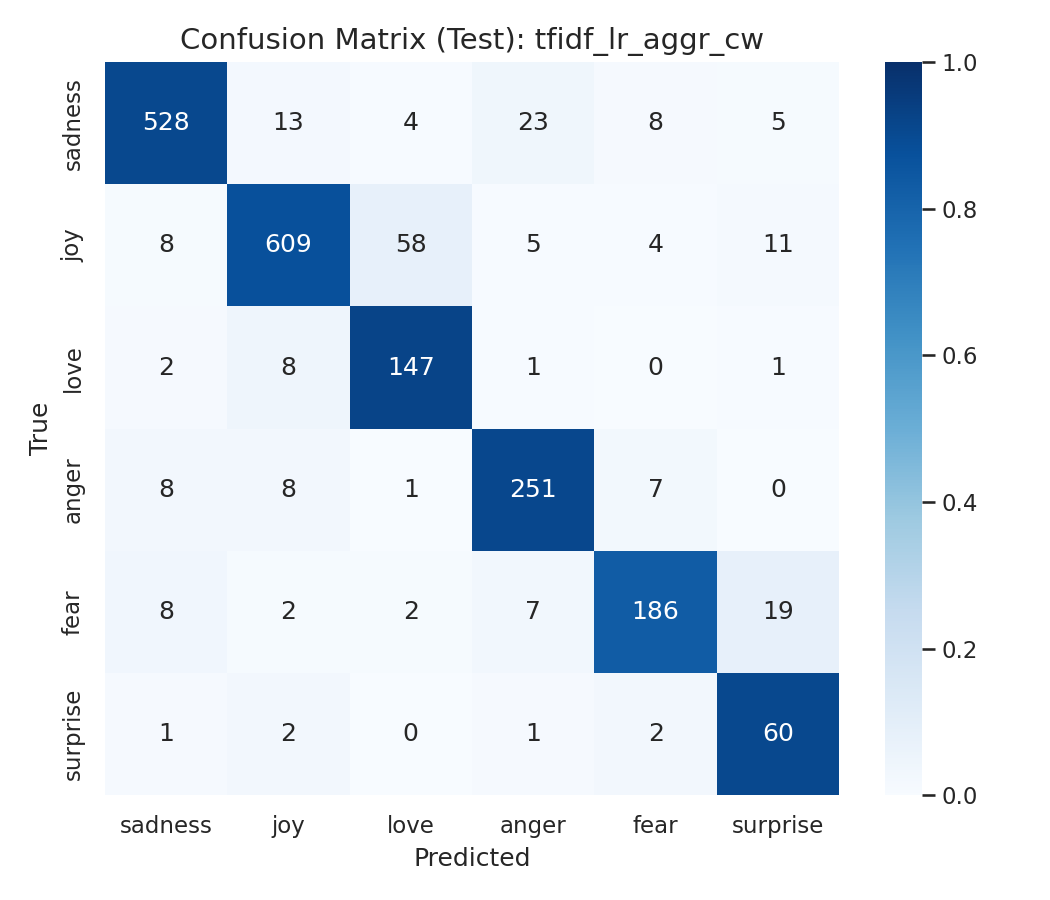
\includegraphics[width=\linewidth]{figures/a2_cm_test_tfidf_lr_aggr_cw.png}\par{\fontsize{6}{7}\sbf\selectfont Baseline \mut{0.8548}}\end{card}
  \begin{card}[left=2pt,right=2pt,top=2pt,bottom=3pt]\centering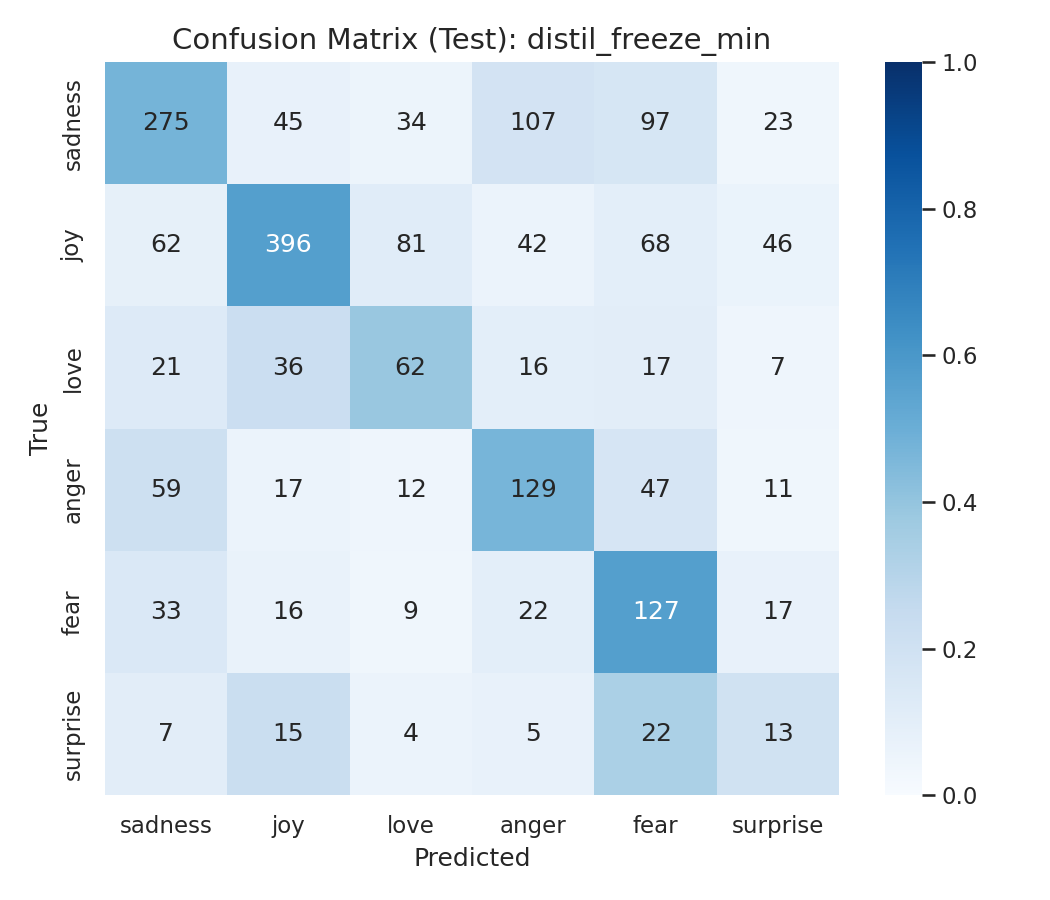
\includegraphics[width=\linewidth]{figures/a2_cm_test_distil_freeze_min.png}\par{\fontsize{6}{7}\sbf\selectfont Frozen \mut{0.4199}}\end{card}
\end{tcbraster}
\end{frame}

\begin{frame}{All 12 runs on test}
\vskip0pt
\begin{card}[left=5pt,right=5pt,top=3pt,bottom=3pt]
  {\fontsize{6.6}{7.6}\selectfont\renewcommand{\arraystretch}{1.12}
  \begin{tabularx}{\linewidth}{@{}llYcccc@{}}
    \toprule
    \thd{Model} & \thd{Setup} & \thd{Seed} & \thd{Val F1} & \thd{Test Acc} & \thd{Test F1} & \thd{Test $-$ Val}\\
    \midrule
    \hl {\sbf DistilBERT} & {\sbf full (selected)} & 42 & 0.9148 & 0.9270 & {\sbf 0.8902} & $-$0.0246\\
    DistilBERT & full & 43 & 0.9178 & 0.9230 & 0.8854 & $-$0.0324\\
    DistilBERT & full & 44 & 0.9140 & 0.9245 & 0.8828 & $-$0.0313\\
    BERT & full & 42 & 0.9200 & 0.9280 & 0.8881 & $-$0.0318\\
    BERT & full & 43 & 0.9145 & 0.9245 & 0.8877 & $-$0.0268\\
    BERT & full & 44 & 0.9145 & 0.9270 & 0.8874 & $-$0.0271\\
    TF-IDF + LR & aggressive, weights (selected) & -- & 0.8758 & 0.8905 & 0.8548 & $-$0.0210\\
    TF-IDF + LR & minimal, weights & -- & 0.8489 & 0.8695 & 0.8365 & $-$0.0124\\
    TF-IDF + LR & minimal, no weights & -- & 0.7527 & 0.8325 & 0.7289 & $-$0.0239\\
    DistilBERT & frozen & 42 & 0.4186 & 0.5010 & 0.4199 & +0.0013\\
    DistilBERT & frozen & 43 & 0.4132 & 0.4940 & 0.4199 & +0.0066\\
    DistilBERT & frozen & 44 & 0.4253 & 0.4970 & 0.4233 & $-$0.0020\\
    \midrule
    \mut{Majority (joy)} & -- & -- & \mut{0.0868} & \mut{0.3475} & \mut{0.0860} & --\\
    \bottomrule
  \end{tabularx}}
\end{card}
\end{frame}

\end{document}
